\documentclass[standalone, version=2.0]{huangfusl-template}
\begin{document}
    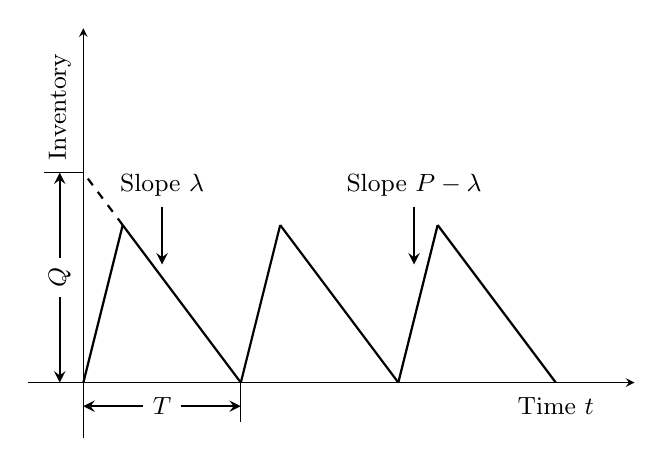
\begin{tikzpicture}
        [
            Axis/.style={-stealth},
            Plot/.style={thick},
            Fill/.style={fill=grey!20},
            Notation/.style={thick, -stealth},
            VLabel/.style={rotate=90, font=\small},
            HLabel/.style={font=\small}
        ]
        \draw[Axis] (-0.7, 0) -- (7, 0);
        \draw[Axis] (0, -0.7) -- (0, 4.5);
        \foreach \x in {1, 2, 3} {
            \draw[Plot] (2 * \x - 2, 0) -- (2 * \x - 1.5, 2);
            \draw[Plot] (2 * \x - 1.5, 2) -- (2 * \x, 0);
        }
        \draw[Plot, dashed] (0.5, 2) -- (0, 8 / 3);
        \draw (2, -0.5) -- (2, 0);
        \draw (-0.5, 8 / 3) -- (0, 8 / 3);
        \node[HLabel] (Label_T) at (1, -0.3) {$T$};
        \draw[Notation] (Label_T) -> (0, -0.3);
        \draw[Notation] (Label_T) -> (2, -0.3);
        \node[VLabel] (Label_Q) at (-0.3, 4 / 3) {$Q$};
        \draw[Notation] (Label_Q) -> (-0.3, 0);
        \draw[Notation] (Label_Q) -> (-0.3, 8 / 3);
        \node[HLabel] (XLabel) at (6, -0.3) {Time $t$};
        \node[VLabel] (YLabel) at (-0.3, 3.5) {Inventory};

        \node[HLabel] (Slope1) at (1, 2.5) {Slope $\lambda$};
        \draw[Notation] (Slope1) -> (1, 1.5);
        \node[HLabel] (Slope2) at (4.2, 2.5) {Slope $P - \lambda$};
        \draw[Notation] (Slope2) -> (4.2, 1.5);
    \end{tikzpicture}
\end{document}